\chapter{THE CONTINUUM}
% !TEX root = hazy2.tex

\section{Overview}

Under most circumstances the radiation field produced by the central object
is the only source of heat and ionization.
This section describes how this
continuum is treated.

\section{Attenuation of the incident continuum}

In an \cdTerm{open geometry} scattering attenuates the incident continuum as
\begin{equation}
I = {I_o}{\left( {1 + 0.5\,d{\tau _{scat}}} \right)^{ - 1}}.
\end{equation}
Scattering does not affect the continuum in a \cdTerm{closed geometry}.
Absorption attenuates the incident continuum as
\begin{equation}
I = {I_o}\exp ( - d{\tau _{abs}}).% (2)
\end{equation}
for both geometries.

\section{Recombination equilibrium}

\subsection{On-the-spot approximation}

A modified version of the ``on-the-spot'' (OTS) approximation is used
in the treatment of sources of diffuse ionizing radiation when the \cdCommand{diffuse OTS} command is used.
Were no other opacity sources present, then, for a
closed geometry that is optically thick in the Lyman continuum, all
recombinations of hydrogen or helium to the ground state would produce
ionizing photons.
Other atoms of the recombined species would quickly absorb
these.
In this case OTS is an excellent approximation (\citealp{VanBlerkom1967,Baessgen1988}).
However, other
opacity sources are present, and these compete in absorbing protons produced
by recombinations, making the recombination process more efficient than
the OTS approximation would suggest.

The recombination coefficients are modified by the presence of all other
opacity sources, such as grains, free-free or \hminus\ absorption,
and the heavy element opacities, in the following manner.
The net effective recombination
rate coefficient (cm$^3$~s$^{-1}$) to level $n$,
$\hat{\alpha} ({T_e},n)$,
is written in terms of the spontaneous radiative recombination rate
coefficient $\alpha ({T_e},n)$ and the opacities (cm$^{-1})\,\kappa_n$
and $\kappa_o$ for the level $n$ and other opacity
sources respectively, as
\begin{equation}
\hat \alpha \left( {{T_e},n} \right) = \alpha ({T_e},n)\left\{ {{P_c}(n)
+ \left[ {1 - {P_c}(n)} \right]\left( {\frac{{{\kappa _o}}}{{{\kappa _o}
+ {\kappa _n}}}} \right)} \right\},
\end{equation}
where $P_c(n)$ is the continuum escape probability.
In general, $P_c(n)$ varies
between 0 and 0.5 for an optically thick open geometry
(see, for example
\citealp{Davidson1977}), $P_c \sim 1$ if the gas is optically thin,
and $P_c \sim 0$ for ground
states if the gas is optically thick and the geometry is closed.  All
computed opacity sources are included in $\kappa_o$.

These recombination continua produce a flux of local on-the-spot photons,
$\varphi_{OTS}$ (cm$^{-2} \ps$).
The OTS photoabsorption rate
$\Gamma_{OTS}$ (s$^{-1}$), used to determine
the ionization or heating rate for the gas or grain constituents,
is then
$\Gamma_{OTS} = \alpha_\nu \varphi_{OTS}$ where $\alpha _\nu$ is the
absorption cross section at frequency $\nu$.
The OTS
flux is related to the spontaneous recombination rate coefficient by
\begin{equation}
{\varphi _{OTS}} = \alpha \left( {{T_e},n}
\right)\;{n_e}\,{n_{ion}}\;\left[ {\frac{{1 - {P_c}(\tau )}}{{{\kappa _o}
+ {\kappa _n}}}} \right]\;\;{{\mathrm{cm}}^{ - 2}}\;\ps
\end{equation}
where $n_{ion}$ is the density of the ion.
These are stored in the
vectors \cdVariable{otscon} and \cdVariable{otslin},
which map one-to-one onto the vectors \cdVariable{flux} and
\cdVariable{anu}.

\subsection{Outward only approximation}

A composite ``outward-only'' (\citealp{Tarter1967}) --``on-the-spot''  approximation
is used in the treatment of sources of diffuse ionizing radiation when the
\cdCommand{diffuse outward} command is used.
This is the default assumption.
The
escaping radiation is then propagated in the outward direction (all for
the spherical case, and half for an open geometry).

\section{Continuous opacities}

The cloud is divided into a large number of concentric shells (zones)
and the attenuated and diffuse continua and physical conditions are then
determined within each.

The main opacity sources in the ultraviolet continuum are generally
photoelectric and free-free (inverse bremsstrahlung) absorption,
grain opacity,
electron scattering (of both bound and free electrons), and the damping
wings of Lyman lines (Rayleigh scattering).
The main reemission mechanisms
are generally free-free (bremsstrahlung), grain emission, free-bound, and
two-photon emission.  Grains are not present by default but can be added
as an option.  Continuous absorption and reemission by all ground states,
and many excited states,
of all ionization stages of the \LIMELM\ elements in
the calculation are explicitly included.
Great care is taken to ensure
that each absorption mechanism is balanced by a reemission process, and
vice versa, so that energy balance in the strict thermodynamic equilibrium
limit can be achieved.

\subsection{Total opacity arrays}

Total absorption opacities (cm$^{-1}$) are storied in the vector
\cdVariable{opac}.
Total
scattering opacities (cm$^{-1}$) are stored in \cdVariable{scatop}.
The opacities are
evaluated in routine \cdRoutine{ConvIonizeOpacityDo} and are within the
\cdVariable{opac} structure
(defined in \cdFilename{opacity.h}).

\subsection{Cross-section array}

\emph{Storage.} The cross sections per particle (cm$^2$) for individual species
(atoms, ions, molecules, etc) are stored within the array \cdVariable{OpacStack}, a stack
array with a single dimension.  These cross sections are evaluated when
the code is initialized in routine \cdRoutine{OpacityCreateAll}.

\emph{Array indices.}  Each species has an associated array index
that defines
the offset between the origin of \cdVariable{OpacStack},
the frequency array
\cdVariable{anu}, and
the opacity at the threshold.
If this offset has the name \cdVariable{ioff}, for
instance, then the cross section at threshold will be given by array element
\cdVariable{OpacStack[ioff]}.  If \cdVariable{ip} is the index to the threshold energy within \cdVariable{anu},
then the array index to the cross section at energy $i$ will be $i-ip+ioff$.

\emph{Individual cross-sections.}  The function \cdRoutine{csphot}
returns the cross section
at a specific frequency for any species.
It has three arguments, 1) the
pointer to the frequency in \cdVariable{anu} where the cross section
is to be evaluated,
2) the pointer to the threshold for the species, and 3) the \cdVariable{ioff} offset
described above.
All are integer variables.

\subsection{Photoionization rates}

Photoionization rates (units s$^{-1}$) can be computed by several functions.
Which is used at a particular time is determined by circumstances.
\begin{description}
\item[GammaK]  This computes the photoionization rate with
allowance for an
arbitrary fluorescence yield.
This routine is a major pacesetter for the
code since it is used to evaluate the continuum rates
in the majority of
the cases.
The photoionization rate is given by
\begin{equation}
{\Gamma _n} = 4\pi \,\int_{{\nu _o}}^\infty  {\frac{{{J_\nu }}}{{h\nu
}}\;{\alpha _\nu }\;d\nu }  \quad [\mathrm{s}^{-1}].% (5)
\end{equation}
where $\alpha _\nu$ is the photoionization cross section [cm$^{-2}$].  The routine has three
integer arguments, the \cdVariable{anu} pointers to the lower and upper energies and
the offset to the opacity array \cdVariable{ioff} (described above).

\item[GammaPrt]   This is a special version of \cdRoutine{GammaK}
that writes the step by step results of the integration on any open file.  The output lists the
product of the photon flux and the cross section,
the photon flux, and the opacity.

\item[GammaBn]   This is a special version of \cdRoutine{GammaK}
that is used when the
correction for stimulated emission or induced recombination is important.
The photoionization rate is given by
\begin{equation}
{\Gamma _n} = 4\pi \,\int_{{\nu _o}}^\infty  {\frac{{{J_\nu }}}{{h\nu
}}\;{\alpha _\nu }\;d\nu }\quad[\mathrm{s}^{-1}]% (6)
\end{equation}
and the rate for induced recombination and its associated cooling is computed
as
\begin{equation}
\alpha \left( {ind} \right) = P_n^*4\pi \int_{{\nu _o}}^\infty
{\frac{{{J_\nu }}}{{h\nu }}\;{\alpha _\nu }\exp \left( { - h\nu /kT}
\right)\;d\nu } \quad [\mathrm{cm}^3 \; \mathrm{s}^{-1}].% (7)
\end{equation}
where $P^*$ is the LTE population.

\item[GammaPrtRate] will print photo rates for all shells
of an ion and element.
It is called with three arguments, a file handle,
followed by the ionization
stage and element number on the C scale (0 for H or atoms, etc).
\end{description}

\subsection{Attenuation within the zone}

A correction must be made to account for the attenuation of the continuum
across the zone \citep{Netzer1984}.
Assuming that the continuum
varies across the zone as
\begin{equation}
\frac{{I(\nu ,\,\delta r)}}{{{I_o}(\nu )}} = \exp \left( { - \kappa \left(
\nu  \right)\,f(r)\,\delta r} \right)% (8)
\end{equation}
then the intensity averaged over a zone with thickness $\delta r$ is
\begin{equation}
\left\langle {\frac{{I\left( {\nu ,\delta r} \right)}}{{{I_o}(\nu )}}}
\right\rangle  = \frac{{1 - \exp \left( { - \kappa \left( \nu
\right)\,f(r)\,\delta r} \right)}}{{\kappa \left( \nu  \right)\,f(r)\,\delta
r}}% (9)
\end{equation}
where $\kappa(\nu)$ is the absorption opacity and $f(r)$ is the filling factor.  The
coefficients giving this ratio as a function of energy are stored in the
vector \cdVariable{tmn}, and are evaluated in routine \cdRoutine{radinc}.  The continuum stored
in \cdVariable{flux} is multiplied by these factors
in the same subroutine.

\subsection{Rayleigh scattering}

Clouds with neutral hydrogen column densities greater than
$10^{23}\, \mathrm{cm}^{-2}$
are optically thick to Rayleigh scattering at wavelengths near L$\alpha $, and this
process is a major scattering opacity source at short wavelengths for
grain-free environments.

Rayleigh scattering cross sections given by \citet{Gavrila1967} are used,
joined with expressions for the radiative damping wings of Lyman lines
(\citealp{Mihalas1978}).
For wavelengths longward of 1410 \AA\  a power-law fit to
Gavrila's quantal calculations is used;
\begin{equation}
{\sigma _{Ray}} = 8.41 \times {10^{ - 25}}{\varepsilon ^4} + 3.37 \times
{10^{ - 24}}{\varepsilon ^6} + 4.71 \times {10^{ - 22}}{\varepsilon
^{14}}\quad {\mathrm{c}}{{\mathrm{m}}^2}% (10)
\end{equation}
where $\varepsilon \equiv /cR_\infty$ is the photon energy in Rydbergs.  This fit is accurate to
typically a percent, with occasional errors as large as 4 percent.

For wavelengths between 1410 \AA\  and the Lyman limit, radiative
broadening of the Lyman lines is assumed (\citealp{Mihalas1978});
\begin{equation}
{\sigma _{Ray}} = \sum\limits_{i = 2}^4 {\left(
{\frac{{q_e^2\,{f_{1,i}}}}{{{m_e}c}}} \right)} \frac{{\Gamma /4\pi
}}{{{{\left( {\nu  - {\nu _{1,i}}} \right)}^2}}}\quad {\mathrm{c}}{{\mathrm{m}}^2}% (11)
\end{equation}
where $\Gamma$ is the reciprocal lifetime of the upper level $i$ and the sum is over
the first four Lyman lines.  This expression gives cross sections in
excellent agreement with \citet{Gavrila1967} for these wavelengths.

\subsection{Free-free opacity}

The main opacity source in the infrared-radio spectral region for many
conditions is free-free opacity with a cross section given by
\begin{equation}
{\alpha _\nu }(ff) = 3.69 \times {10^8}\;{\bar g_{III}}\left( {\nu ,T}
\right)\;f(r)\;{\nu ^{ - 3}}\;{T^{ - 1/2}}\left\{ {1 - \exp \left( { - h\nu
/kT} \right)} \right\}\;\sum\limits_A {} \sum\limits_z {{z^2}\;n_A^{ + z}}
\quad [\mathrm{cm}^{-2}]% (12)
\end{equation}
(see, for example, \citealp{Mihalas1978}).
The sum is over all ions $n^{+z}$ of element
$A$ and over all elements.
The temperature averaged gaunt factor
${\bar g_{III}}(\nu ,T)$
is taken from \citet{Hummer1988} (see also \citealp{Karzas1961}) and are
evaluated in routine \cdRoutine{gffsub} that was originally written by D. Hummer.

This routine did not extend to energies that could be treated by
asymptotic expansions of the gaunt factor.
\cdRoutine{gffsub} was modified by
J.~Ferguson to extend over the full temperature and energy range considered
by \Cloudy, and later extensively rewritten by Ryan Porter.
Figure \ref{fig:FreeFreeGauntFactors} shows
the gaunt factors as functions of photon energy and temperature.

\begin{figure}
\centering
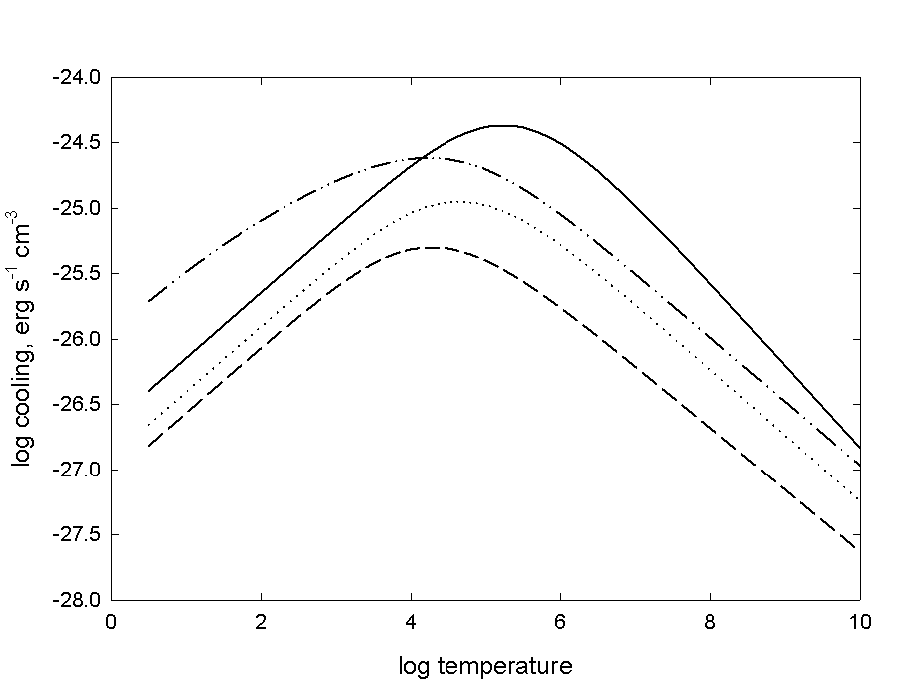
\includegraphics[scale=0.8]{FreeFreeGauntFactors}
\caption[free-free gaunt factors]
{\label{fig:FreeFreeGauntFactors}Thermally averaged
free-free gaunt factor.  The gaunt factor is
shown as a function of photon energy and temperature.}
\end{figure}

\subsection{Bound-free opacity}

Continuum optical depths for photoabsorption from level l are given by
\begin{equation}
d{\tau _l}\left( \nu  \right) = {\alpha _\nu }\left( n
\right)\;{n_l}\,\left[ {1 - \exp \left( { - h\nu /kT} \right)/{b_l}}
\right]\;f(r)\;\delta r% (13)
\end{equation}
where $b_l$ is the departure coefficient for level $l$ and $\alpha _\nu$ is the absorption
cross section [cm$^{-2}$].

\subsection{Plasma frequency}

The plasma frequency, the energy where the index of refraction of an
ionized medium goes to zero, is given by
\begin{equation}
{\nu _{pl}} = {\left( {\frac{{{n_e}q_e^2}}{{\pi \,{m_e}}}} \right)^{1/2}}
= 8.978 \times {10^3}\,n_e^{1/2}\;{s^{ - 1}} = 2.729 \times {10^{ -
12}}\;n_e^{1/2}\;{\mathrm{Ryd}}%. (14)
\end{equation}
An ionized gas will reflect the incident continuum for energies smaller
than this.  This shielding becomes important for the energy range considered
by \Cloudy\ for electron densities greater than $\sim 10^7 \mathrm{cm}^{-3}$.  For higher densities
this process is treated by setting the intensity of the incident continuum
to zero for energies below the plasma frequency, adding this portion of
the incident continuum to the reflected continuum, and not allowing emission
or absorption for any processes that occur below the plasma frequency.

\subsection{Pressure lowering of ionization potential}

The electric field of nearby charges in the continuum acts to lower the
ionization potential.  The amount by which it is lowered is determined by
the electron density.
Ryan Porter extended the code to consider all species
treated with the iso-electronic model atoms.
\section{Continuum range}

The energy interval \emm\ $-$ \egamry\ is divided into a
large number of energy cells with nearly logarithmically increasing widths.

\section{The continuum mesh}

\subsection{Continuum mesh logic}

The central frequencies of two cells are related by
\begin{equation}
\frac{{{\nu _{i + 1}}}}{{{\nu _i}}} = \exp(r)% (100)
\end{equation}
where $r$ is the resolution, $\delta \nu/\nu$.
Then the $n^{th}$ cell energy is related to
the first cell energy by
\begin{equation}
{\nu _n} = {\nu _0}\,\exp(nr).% (101)
\end{equation}
The cell corresponding to energy $\nu_n$ is then
\begin{equation}
n = \frac{\log(\nu_n/\nu_0)}{r}.
\end{equation}

\subsection{Defining the continuum energy mesh}

The array \cdVariable{anu} gives the energy of the center of each
continuum cell, in Rydbergs.
This energy scale is defined in routine
\cdRoutine{ContCreatePointers}.

\subsection{Changing the energy resolution of the mesh}

The file \cdFilename{continuum\_mesh.ini} contains ordered pairs
of continuum energies
and resolving powers (defined as $1/r$) that are read by \cdRoutine{ContCreatePointers}
to set the continuum
mesh when calling \cdRoutine{fill}.
Change the contents of
\cdFilename{continuum\_mesh.ini} to change
the resolution of the continuum mesh.
The file explains how to do this.

If the energy resolving power is increased then the code will require more
mesh points to cover the full continuum and will run more slowly, but the
predicted continuum will have greater detail.

\section{Continuum generation}

The continuum is generated by the function \cdRoutine{ffun}.
\cdRoutine{ffun} has a single argument,
the energy in Rydbergs, and it returns the number of photons per
unit area, time, and Rydberg, at that energy.
\cdRoutine{ffun} sums over all the
specified continua and applies the appropriate normalization factors.
Another function, \cdRoutine{ffun1},
evaluates each individual continuum, and is normally
called only by \cdRoutine{ffun}.

The units, and their conversion to other measures of the continuum, are
given below.  The photon flux density is:
\begin{equation}
{\varphi _\nu }(\nu ) = \mathrm{ffun}(\nu )\quad [\mathrm{photons\,
cm}^{-2} \, \mathrm{s}^{-1} \, \mathrm{Ryd}^{-1}] .
\end{equation}
This is stored in the photon array:
\begin{equation}
flux({\nu _i}) = {\varphi _\nu }(\nu )\;\delta {\nu _i} = \mathrm{ffun}({\nu _i})
\times widflx(\nu )\quad [\mathrm{photons\, cm}^{-2}\, \mathrm{s}^{-1}]
\end{equation}
where \cdVariable{widflx} is an array containing the width of
each continuum bin.
Finally, the energy flux density is given by
\begin{equation}
{f_\nu }(\nu ) = {\mathrm{ffun}}(\nu )\;h\left( {\frac{\nu }{{{\nu _{912}}}}}
\right)\quad
 [\mathrm{erg\, cm}^{-2}\, \mathrm{s}^{-1}\, \mathrm{Hz}^{-1}]
\end{equation}
and
\begin{equation}
\nu {f_\nu }(\nu ) = {\mathrm{ffun}}(\nu )\;h\left( {\frac{\nu }{{{\nu
_{912}}}}} \right){\nu _{912}}\,h{\nu _{Ryd}}\quad
[\mathrm{erg\, cm}^{-2}\, \mathrm{s}^{-1}].
\end{equation}

\section{Energy units; the Rydberg}

Continuum energies are usually given in Rydbergs.
The energy of level
$n$ of a hydrogenic atom is given~by
\begin{equation}
{E_n} =  - \frac{{\cal R}_{\mathrm{H}}}{{{n^2}}}, n = 1,2,3,\ldots,\quad [\mathrm{units\ of\
}\mathcal{R}_{\mathrm{H}}]
\end{equation}
where the Rydberg energy is given by
\begin{equation}
{\cal R} = \frac{{\mu q_e^4}}{{2{\hbar ^2}}} = \frac{\mu }{{{m_e}}}{{\cal
R}_\infty }
\end{equation}
and the reduced mass of the orbiting electron $\mu$ is related
to the electron
and nuclear mass $m_e$ and $m_{nuc}$ by
\begin{equation}
\mu  = \frac{{{m_e}{m_{nuc}}}}{{{m_e} + {m_{nuc}}}} = \frac{{{m_e}}}{{1
+ {{{m_e}} /{{m_{nuc}}}}}}\quad  [\mathrm{g}],% (109)
\end{equation}
(\citealp{Friedrich1998}).
Note that as ${m_{nuc}} \to \infty $, $\mu  \to {m_e}$.
This Rydberg energy $\cal{R}_{\mathrm{H}}$ is smaller than
the energy for an infinite mass
nucleus $\cal{R}_\infty$  by the ratio $\mu/m_e$.
Using the 1998 CODATA revision of the
fundamental constants (see \citealp{Cohen1987,Mohr1998}) the
infinite mass Rydberg energy is given by
\begin{equation}
{{\cal R}_\infty } = \frac{{{m_e}q_e^4}}{{2{\hbar ^2}}} = 13.605698
  [\mathrm{eV}]
\end{equation}
and
\begin{equation}
\begin{array}{c}
 {{\cal R}_\infty }/\left( {2\pi \hbar c} \right) =
109737.315686\;{\mathrm{c}}{{\mathrm{m}}^{ - 1}} \\
 {{\cal R}_\infty }/\left( {2\pi \hbar } \right) = 3.28984196038 \times
{10^{15}}\;{\mathrm{Hz}} \\
 \left( {2\pi \hbar c} \right)/{{\cal R}_\infty } = 91.126732\;{\mathrm{nm}} \\
 \end{array}.
\end{equation}
The ionization potential of hydrogen $\cal{R}_{\mathrm{H}}$ is  $\mu/m_e$ or
$\sim 0.99946$ times
smaller than $\cal{R}_\infty$.
\footnote{$\cal{R}_{\mathrm{H}}$ was the Rydberg unit used by \Cloudy\ before 1988.}
We have
\begin{equation}
\begin{array}{c}
{\cal{R}_{\mathrm{H}}} = 13.59842\;\eV\\
{\cal{R}_{\mathrm{H}}} = 2.178728\times 10^{11}\;\erg\\
\left( 2\pi \hbar\right)/{\cal{R}_{\mathrm{H}}} = 91.176430\;{\mathrm nm}\\
{\cal{R}_{\mathrm{H}}} = 109677.576\;{\mathrm cm}^{-1}
\end{array}
\end{equation}
The difference between $\cal{R}_{\mathrm{H}}$ and $\cal{R}_\infty$ is
significant since it enters as the third
power in the photon phase-space conversion factor $2h \nu^3/c^2$.

The Bohr radius is for an infinite mass nucleus is given by
\begin{equation}
\begin{array}{l}
 {a_o} = {{{\hbar ^2}}/
\left( {{m_e}q_e^2} \right)} = 0.5291772083
\times {10^{ - 8}} \\
 a = {{{a_o}} /\mu } \\
 \end{array}[\mathrm{cm}].
\end{equation}
In the ``atomic units'' system of measuring quantities lengths are given
in terms of the Bohr radius and energies in ``Hartree'' units.  One Hartree
is twice the Rydberg energy.
